
\chapter{Návrh a implementácia}
\label{kap:implementacia}

V kapitole opisujeme priebeh vzniku aplikácie, implementačné detaily, postupy a rozhodnutia. Základné členenie obsahu je podľa modulov, za ktoré považujeme celky aplikácie ako editor kódu v grafickom jazyku, modul pre sériovú komunikáciu či modul pre simuláciu. Súčasťou sú tiež implementačne zmeny v riadiacom programe robota.

Vývoj začíname návrhom systému, ktorý umožní v aplikácii spístupniť rôzne programovacie verzie pre rôzne modely robota a rôzne typy riadiaceho programu. Pokračujeme návrhom kostry a vizuálnej podoby aplikácie, v ktorej neskôr vzniknú jednotlivé moduly. V prvej fáze implementujeme časti podporujúce komunikáciu s aktuálnou verziou riadiaceho programu robota Otto a jeho programovanie. Nasleduje etapa rozširovania funkcionalít (hlavne grafického jazyka)  a práca na module simulácie.

K orientácii v štruktúre aplikácie môže byť nápomocný obrázok \ref{obr:app-structure}, kde sú v stĺpcoch znázornené jednotlivé moduly. Zobrazené sú tiež ich závislosti na technológiách a zdrojových súboroch.

\begin{figure}
\centerline{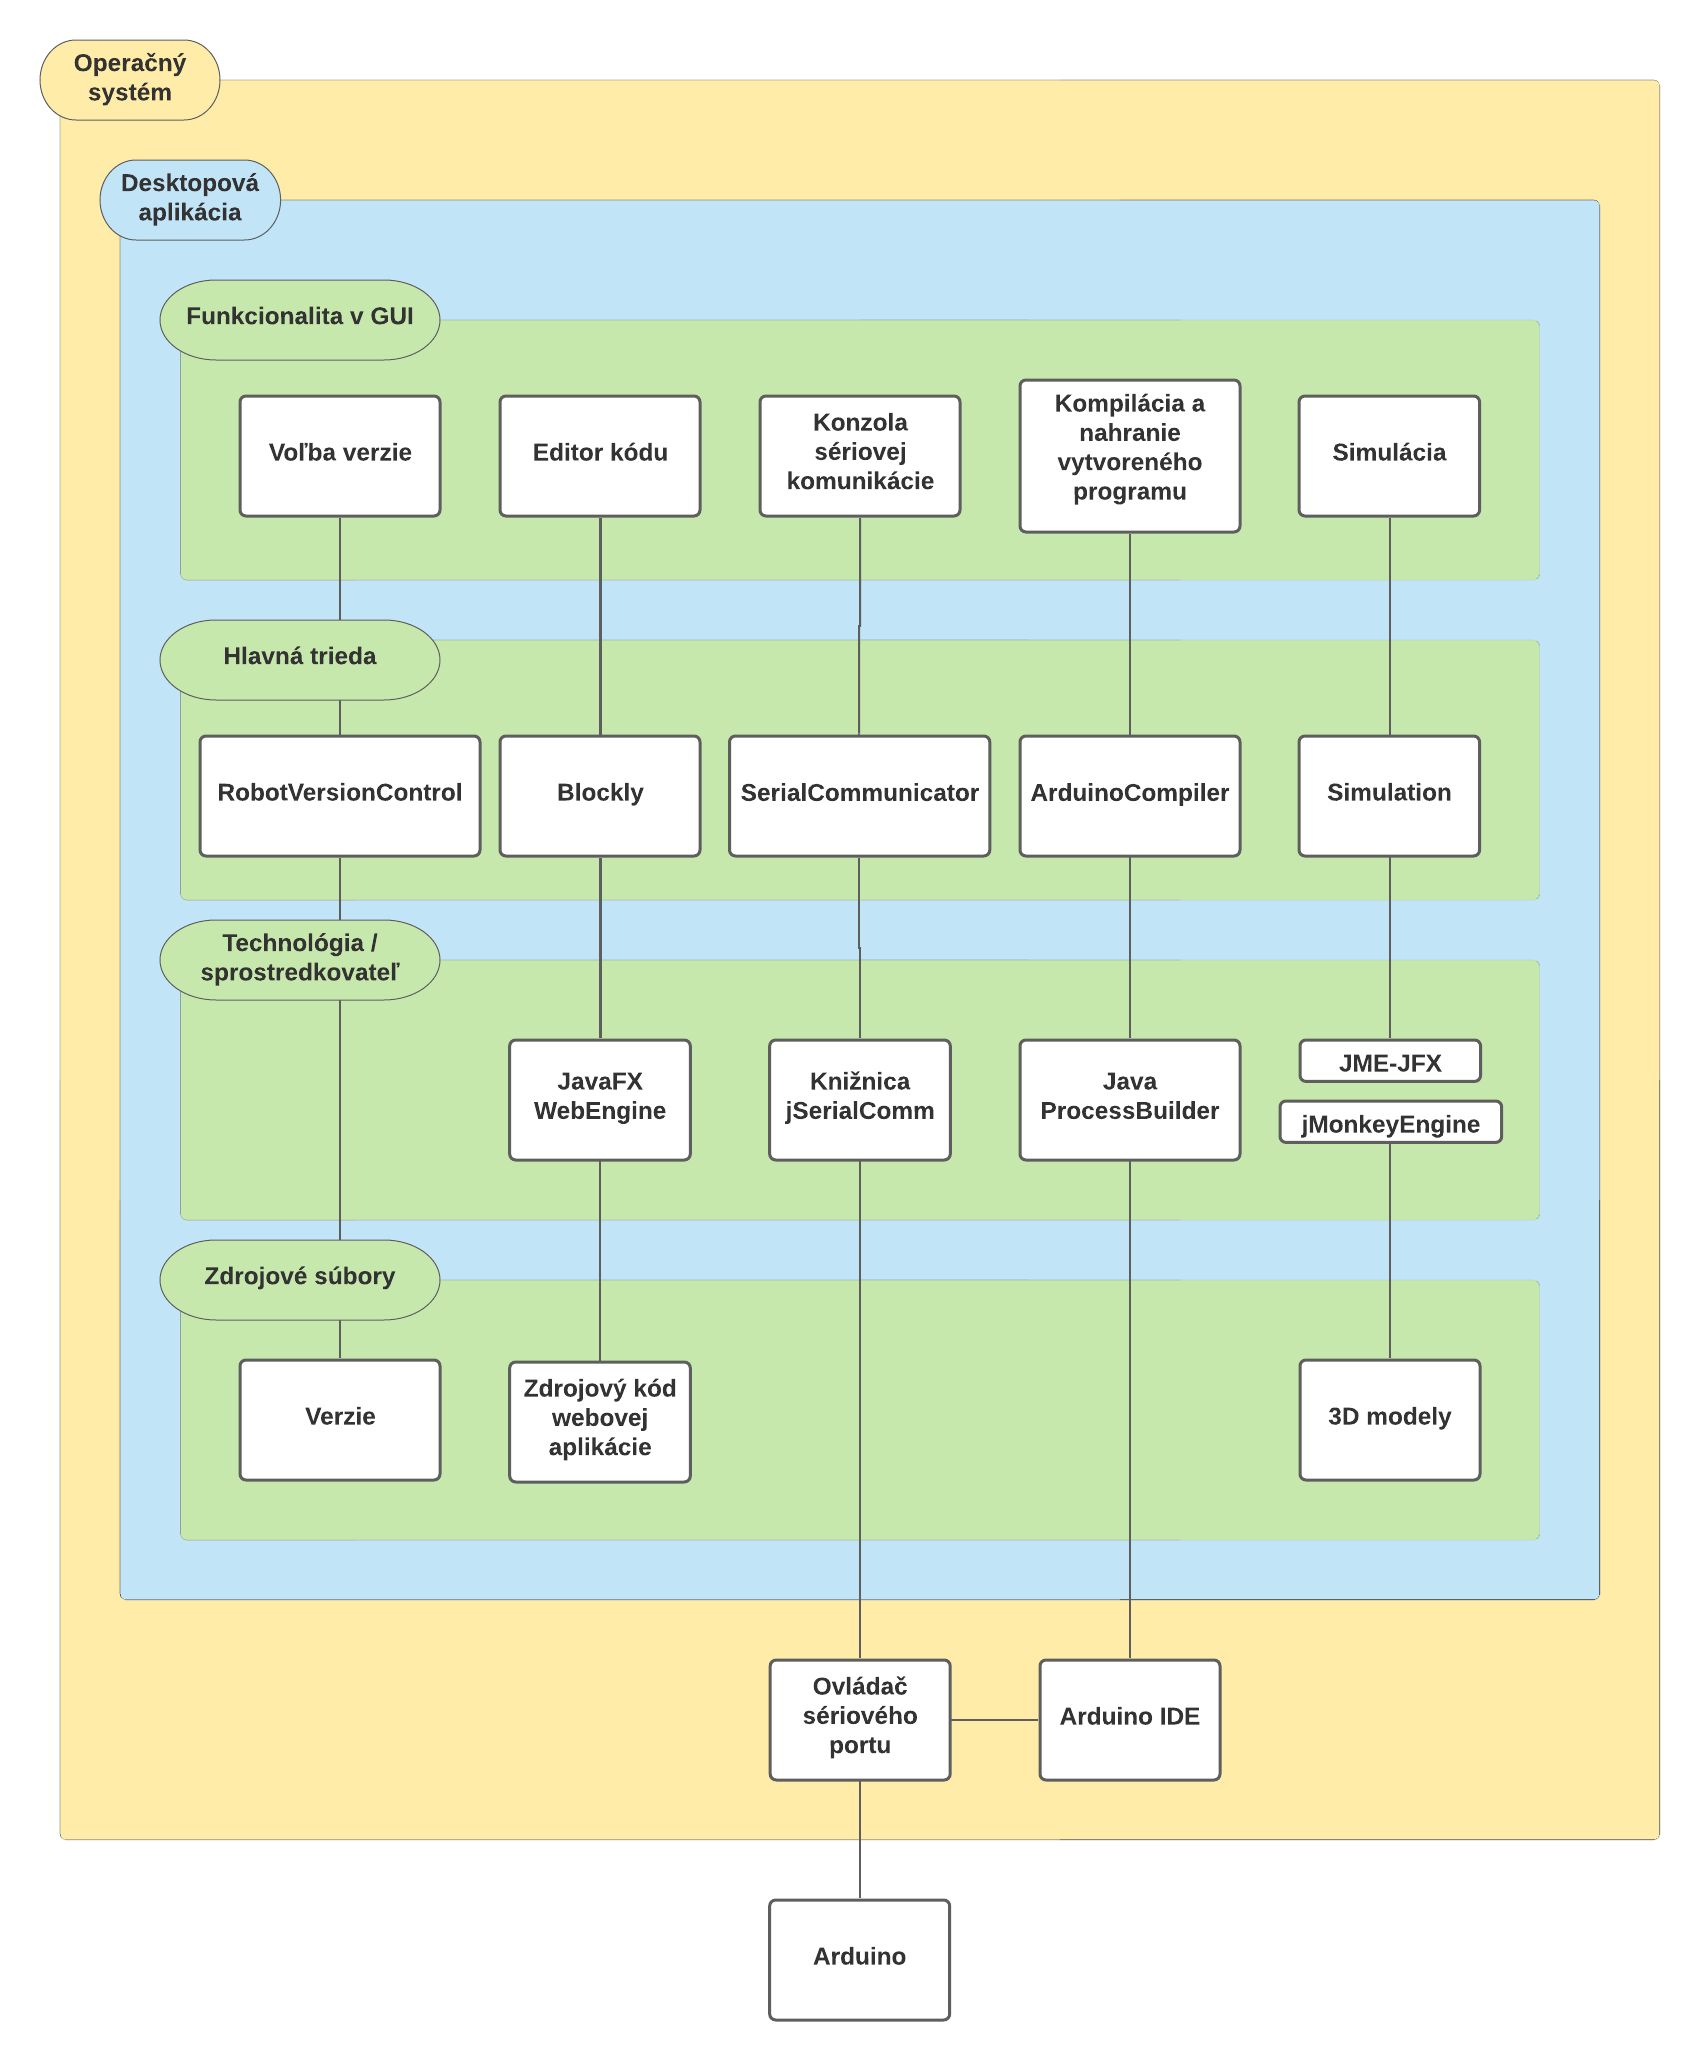
\includegraphics[width=1\textwidth]{images/app-structure}}
\caption[Štruktúra aplikácie]{Štruktúra aplikácie}
\label{obr:app-structure}
\end{figure}


%%%%%
% %%% Modulárny systém
%%%%%
\section{Systém verzií}
Aplikáciu budujeme na systéme verzií. Verziou označujeme súbor údajov určujúcich konfiguráciu aplikácie, podľa ktorej sa správajú (sú dostupné) jednotlivé moduly. Verziu definuje nasledovné:

\begin{itemize}[noitemsep]
\item názov - označenie pre používateľa
\item pre modul editor kódu (Blockly)
\begin{itemize}[topsep=0pt,itemsep=0pt,partopsep=0pt, parsep=0pt]
\item definícia obsahu ponuky zobrazených blokov (obr.\ref{obr:gui-layout}, priestor A)
\item definícia iniciálneho obsahu pracovnej plochy (obr.\ref{obr:gui-layout}, priestor B)
\item označenie generátora kódu (prekladača grafického jazyka)
\end{itemize}
\item pre modul kompilácie a modul sériovej komunikácie
\begin{itemize}[topsep=0pt,itemsep=0pt,partopsep=0pt, parsep=0pt]
\item určenie, či generovaný kód má byť kompilovaný alebo priamo prenášaný sériovou komunikáciou
\end{itemize}
\item pre modul simulácie
\begin{itemize}[topsep=0pt,itemsep=0pt,partopsep=0pt, parsep=0pt]
\item označenie parsera pre vytvorenie inštrukcií pre simuláciu z generovaného kódu
\end{itemize}
\item zoznam logických modulov, pre každý modul:
\begin{itemize}[topsep=0pt,itemsep=0pt,partopsep=0pt, parsep=0pt]
\item názov a opis
\item určenie, či je logický modul povinným
\item určenie súboru s podpornými funkciami modulu
\item veľkosť
\item súvisiace kategórie v ponuke zobrazených blokov modulu editor kódu
\end{itemize}
\item zoznam ukážkových programov, pre každú ukážku:
\begin{itemize}[topsep=0pt,itemsep=0pt,partopsep=0pt, parsep=0pt]
\item názov a opis
\item zoznam použitých logických modulov
\item definíciu (iniciálneho) obsahu pracovnej plochy (obr.\ref{obr:gui-layout}, priestor B)
\end{itemize}
\end{itemize}

Interakcia s aplikáciou začína výberom verzie. V závislosti na jej charaktere môže byť vyžadované skompilovať a nahrať do mikropočítača riadiaci program. Ide napríklad o verziu podporujúcu programovanie robota Otto spôsobom \uv{program reprezentovaný číslami v pamäti RAM} (kapitola \ref{subsub:otto-programovanie}), kde všetka ďalšia interakcia a programovanie prebieha bez nutnosti kompilácie. V inom prípade môže byť používateľovi po voľbe verzie umožnený výber \textit{logických modulov}. Jedná sa o (tematické) celky funkcionalít, príkladom je logický modul \textit{senzory}, ktorý používateľovi sprístupní v grafickom jazyku bloky umožňujúce čítať aktuálne merané hodnoty alebo čakať na nameranie konkrétnej hodnoty. Logické moduly sú tiež previazané s podpornými funkciami, ktoré je nutné kompilovať ako súčasť riadiaceho programu. Logickým modulom je možné v systéme verzií definovať veľkosť a obmedziť tak výber kombinácie prekračujúcej pamäťový limit mikropočítača. Logické moduly tiež umožňujú zjednodušiť programovanie začiatočníkom obmedzením množstva dostupných funkcií. K verziám môžu byť pripojené príklady programov v nich zostrojiteľných.

Počas vývoja aplikácie vznikli dve verzie pre programovanie robota Otto. Verzia umožňujúca tvorbu definíciu choreografií komunikáciou s riadiacim programom vyvinutým pre účely denných táborov (kapitola \ref{subsub:otto-programovanie}) a verzia pre procedurálne programovanie, sprístupňujúca používateľovi interakciu so senzormi a možnosť definície vlastnej logiky programu takmer od základu.


%%%%%
% %%%    GUI
%%%%%
\section{Grafické rozhranie}
GUI aplikácie tvoríme pomocou JavaFX. Cieľom je vytvoriť prehľadné prostredie, v ktorom sa ľahko zorientuje i požívateľ nižšieho veku. Pri rozmiestňovaní jednotlivých prvkov sú nám nápomocné existujúce aplikácie, no zohľadňujeme i rady autorov knižnice Blockly \cite{blocklyBestPractices}, keďže komponent umožňujúci prostredníctvom nej programovať robota je v našej aplikácii dominantným. Z odporúčaní je zrejmé, že plochu pre manipuláciu s prvkami grafického jazyka je žiaduce maximalizovať a neoddeľovať ju od komponentu umožňujúceho tvorbu blokov (prvkov jazyka).

Ďalšie prvky vyžadujúce v aplikácii väčšiu plochu sú najmä výstupné, predovšetkým ide o výstup pre modul simulácie a výstup \uv{prekladača} grafického jazyka na kód následne kompilovaný a odosielaný do riadiacej jednotky robota. Taktiež je nutné zakomponovať do GUI modul pre komunikáciu s robotom, konzolu sériovej komunikácie.

Výsledné rozloženie môžete vidieť na obrázku \ref{obr:gui-layout}. Tvoriť kód v grafickom jazyku možno v časti \textit{A}, umožňujúcej výber blokov, a ich následným umiestňovaním v priestore \textit{B}. Sektor \textit{C} je vyhradený pre výstup modulu simulácie. Časť \textit{D} je zdieľaná modulom sériovej komunikácie a modulom umožňujúcim náhľad do kódu generovaného prekladom grafického jazyka, medzi ktorými možno prepínať. Nad spomínanými oblasťami sa nachádza lišta nástrojov, sprístupňujúcich funkcie ako vyhľadanie a pripojenie sériovj komunikácie či voľbu verzie programovaného riadiaceho programu robota.

Prípadná zmena usporiadania komponentov nie je v JavaXF zdĺhavou záležitosťou a na základe spätnej väzby od budúcich používateľov možno v rozložení dodatočne vykonať úpravy.

\begin{figure}
\centerline{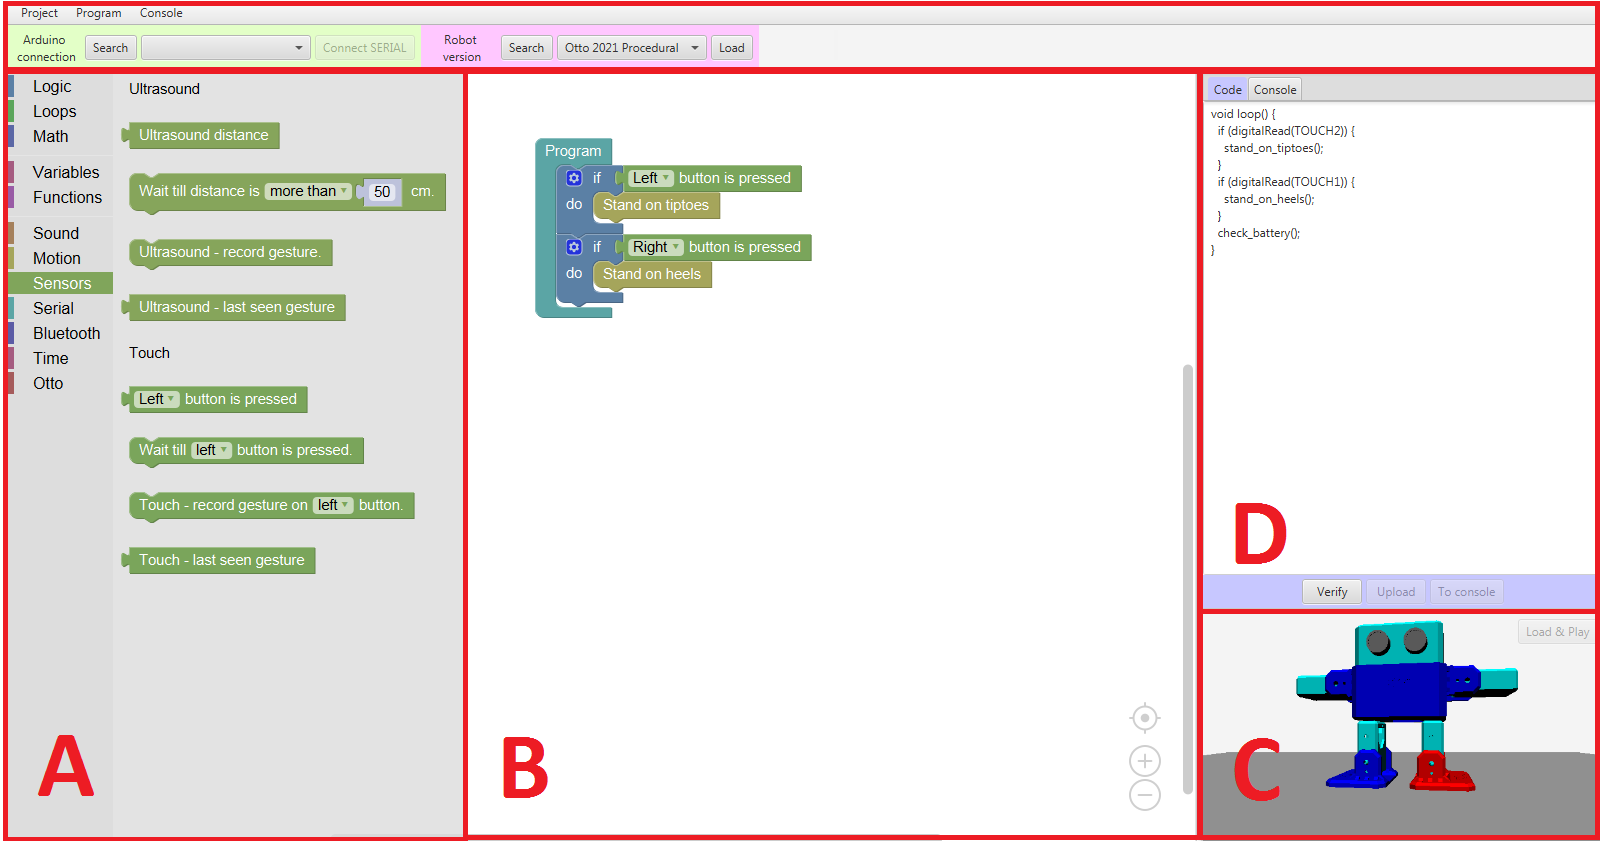
\includegraphics[width=1\textwidth]{images/rozlozenie-gui}}
\caption[Rozloženie používateľského rozhrania]{Rozloženie používateľského rozhrania}
\label{obr:gui-layout}
\end{figure}


%%%%%
% %%% Editor kódu
%%%%%
\section{Editor kódu}
Modul umožňujúci tvorbu (riadiaceho) programu pomocou grafického programovacieho jazyka (GPJ) je v podstate samostatnou webovou JavaScript aplikáciou. V GUI našej aplikácie je zobrazený jej výstup tvorený knižnicou Blockly v komponente WebView (webový prehliadač). Interakcia medzi našou Java aplikáciou a vnorenou \uv{Blockly JavaScript aplikáciou} prebieha pomocou inštancie WebEngine, volaním funkcií navonok poskytnutých knižnicou (umožňujú generovanie kódu práve vytvoreného v GPJ, načítanie obsahu pracovnej plochy, obsahu ponuky blokov a podobne).

%Funkčnosť knižnice je založená na definícii blokov a im prislúchajúcich generátorov. Bloky sú navonok vizuálnym komponentom editora, ich spájaním tvorí používateľ kód. Súčasťou ich definície sú validátory, vykonávajúce kontroly (najmä typové). Validátory určujú obmedzenia použitia blokov, ľubovoľné dva bloky nemusí byť možné spojiť, čím možno vynútiť syntaktické pravidlá cieľového textového programovacieho jazyka. Každému bloku je tiež priradený generátor, ktorý zodpovedá za interpretáciu bloku pri generovaní výsledného kódu (u nás napríklad v jazyku C). Knižnica Blockly poskytuje základné, všeobecné bloky. K dispozícii sú bloky pre \textit{podmienku if}, \textit{cykly}, bloky pre \textit{logické a číselné konštanty} a manipuláciu s nimi (porovnávanie, sčítavanie, negácia a iné), bloky pre \textit{manipuláciu s textom}, \textit{tovrbu zoznamov}, \textit{reprezentáciu a miešanie farieb}, \textit{tvorbu premenných} a \textit{definíciu procedúr a funkcií}. Súčasťou sú generátory pre jazyky JavaScript, Python, Dart, Lua a PHP.

V knižnici dotvárame bloky reprezentujúce funkcie robota umožňujúce pohyb, čítanie hodnôt meraných senzormi, sériovú komunikáciu či komunikáciu rozhraním bluetooth. Komplexitou funkcie poskytovanej blokom je možné nastaviť úroveň abstrakcie. Jednoduchým príkladom je blok \uv{čakania na stlačenie tlačidla} (obrázok \ref{obr:wait-till-couch}). Ľahko ho možno vyskladať z blokov \textit{cyklu while}, \textit{negácie} a bloku pre \textit{načítanie stavu tlačidla}, no najmä pre nižšie vekové kategórie je vhodnejšia alternatíva vyššej abstraktnej úrovene. Iným príkladom je blok pre načítanie gesta pomocou ultrazvukového senzora, ktorý jednoducho reprezentuje v pozadí pomerne zložitú implementáciu časti riadiaceho programu, zabezpečujúcu komunikáciu s hardvérom a elimináciu chyby opakovaným meraním.

\begin{figure}
\centerline{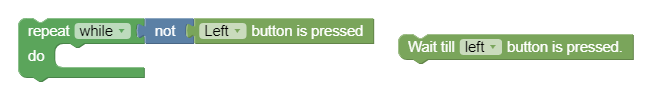
\includegraphics[width=1\textwidth]{images/wait-till-couch}}
\caption[Blockly --- abstrakcia bloku \uv{čakaj na stlačenie tlačidla}]{Blockly --- abstrakcia bloku \uv{čakaj na stlačenie tlačidla}}
\label{obr:wait-till-couch}
\end{figure}

Syntax jazyka C vyžaduje redefiníciu generátorov viacerých prebraných blokov. Vytvárame tiež generátory pre novo konštruované bloky. Usporiadaním v editore kódu sú použité bloky organizované v grafovej štruktúre, generátor je funkcia, ktorej parametrom je blok, na ktorom je volaná. Má prístup k poliam bloku (polia sú prvky pre výber možností, prípadne textový alebo číselný vstup, napríklad blok vpravo na obrázku \ref{obr:wait-till-couch} má pole na výber jednej z dvoch možností, \uv{left} a \uv{right}). Zároveň má generátor prístup k vnoreným blokom (napríklad blok cyklu while má prístup k blokom v tele cyklu) a pripojeným \uv{nasledovníkom} --- bloku pod ním. Návratovou hodnotou je vhodne spracovaný kód so zakomponovaným obsahom potomkov a polí. Kód je generovaný rekurzívne, zvyčajne začínajúc na najvyššom bloku umiestnenom v editore. V našej aplikácii je súčasťou editora fixný blok \uv{program}, ktorý reprezentuje časť \textit{loop} programu v Arduino a kód je tvorený pridávaním blokov do jeho tela. Bloky bez pripojenia (aj nepriameho) k tomuto bloku nie sú pri vyhodnocovaní brané do úvahy. Výnimku majú len bloky umiestnené v tele blokov definujúcich funkcie a procedúry. Príklad možno vidieť na obrázku \ref{obr:disabled-orphan-block}.

\begin{figure}
\centerline{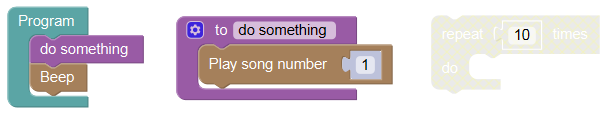
\includegraphics[width=0.65\textwidth]{images/disabled-orphan-block}}
\caption[Blockly --- blok pre riadiaci program robota]{Blockly --- blok pre riadiaci program robota}
\label{obr:disabled-orphan-block}
\end{figure}

Dôležitým komponentom jazyka sú premenné. Blockly je potrebné prispôsobiť pre použitie typových premenných jazyka C, pričom autori podobných aplikácií pristupujú k riešeniu rôzne. V online webovej verzií editora MakeCode (riadenie robota Lego Mindstorms) sú k dispozícii len číselné premenné, textové reťazce a binárne hodnoty môžu byť len konštantou \cite{makeCodeWebEditor}. Na druhej strane, v produkte OttoDIY je možné vytvoriť premennú typu znak, reťazec, celé číslo, desatinné číslo i binárna hodnota. K dispozícií sú bloky pre inicializáciu, priradenie, i získanie hodnoty premennej. Typy nie sú však vizuálne výraznejšie odlíšené. V editore kódu možno deklarovať premennú binárneho typu a následne iným blokom túto premennú inkrementovať, na čo validátor bloku oznámi chybu. Otázne však je, či je vhodné povoliť vytvorenie neprípustného spojenia. V našej aplikácii vynucujeme určenie typu premennej pri jej vytváraní, bez možnosti dodatočnej zmeny. Povolené typy sú celé číslo (int16\_t), textový reťazec (String) a binárna hodnota (bool). Bloky pre priradenie do premennej a čítanie premennej majú v rámci typu rovnakú farbu.



%%%%%
% %%%    Komunikácia, serial
%%%%%
\section{Komunikácia s robotom}
Možnosť komunikácie s robotom je jednou zo základných požiadaviek na našu aplikáciu. Umožňuje vyššiu interakciu s používateľom a je tiež nápomocná pri ladení programov (pomocné výpisy). Komunikácia s robotom na úrovni nahratia kompilovaného programu je predmetom časti \ref{sub:arduinoIDE}, tu je opísaná sériová komunikácia už bežiaceho programu v mikropočítači Arduino s našou aplikáciou. Jedná sa o komplementárnu časť systému k časti implementovanej v mikropočítači (sekcia \ref{sub:arduino}).

\subsubsection{Komunikácia zo strany aplikácie}
V aplikácii je cieľom vytvoriť integrovaný terminál pre sériovú komunikáciu. Mikropočítač Arduino komunikuje po pripojení rozhraním USB a nainštalovaní príslušného ovládača v počítači s OS, ktorý nám toto spojenie sprostredkuje. Podobne pracuje i terminál v Arduino IDE (oficiálne IDE pre vývoj riadiacich programov Arduino) alebo program Putty (klient pre ssh, Telnet, Rlogin a sériovú komunikáciu \cite{putty}). Autori mikropočítača odporúčajú pre implementáciu sériovej komunikácie v Java použitie knižníc \cite{arduinoAndJava}. V článku o prepojení Java --- Arduino sú spomínané dve, údajne nespoľahlivá knižnica RXTX a možná alternatíva, knižnica jSerialComm, ktorú použijeme. 

jSerialComm je platformovo nezávislá knižnica, ľahko integrovateľná do našej aplikácie \cite{jSerialComm}. Umožňuje vyhľadávať pripojené dostupné sérové porty, ako aj obojsmernú komunikáciu po pripojení. Podporuje niekoľko typov operácie, v závislosti na blokovaní čítania z (zápisu do) sériového portu. V prípade čítania sú na výber alternatívy ako \textit{neblokovaná komunikácia}, v ktorej možno príkazom \textit{read()} skúsiť načítať dáta, ak však nie sú k dispozícii (neboli prijaté), vrátený je prázdny reťazec. Inou možnosťou je vynútenie čakania na možný príchod správy a to buď len po nejaký čas alebo až do jej prijatia. Vo všetkých týchto prípadoch by ale v našej aplikácii bolo nutné cyklicky kontrolovať, či nejaké dáta nie sú k dispozícii (ako v mikropočítači), knižnica ale poskytuje vhodnejší prístup, registráciu callback funkcie. Tú knižnica zavolá po každom výskyte špecifikovanej udalosti, ktorom môže byť dostupnosť dát alebo prijatie ucelenej správy. V implementácii volíme možnosť volania callback funkcie po prijatí ucelenej správy, pričom za koniec správy je považovaný znak konca riadku (\textbackslash n --- line feed). Registrovaná callback funkcia správu načíta a zobrazí v termináli používateľovi.

Odosielanie správ je rovnako možné nastaviť do blokujúceho režimu, kde pri pokuse o zápis do sériového portu knižnica čaká buď to určitý čas alebo kým sa podarí odoslať požadovaný počet bajtov. Pre implementáciu volíme neblokovaný prístup, ak používateľ odošle dáta, sú zapísané hneď ako je to možné. Neblokovaný prístup umožní odoslanie viacerých správ, ktoré následne v rovnakom poradí knižnica odvysiela.


%%%%%
% %%%    Kompilácia, upload, Arduino IDE
%%%%%
\section{Kompilácia a nahranie riadiaceho programu}
\label{sub:arduinoIDE}
Kompiláciu a nahranie riadiaceho programu pri vývoji programov pre Arduino zvyčajne zabezpečuje Arduino IDE s grafickým používateľským rozhraním (sekcia \ref{sub:arduino}). Nahrávanie kompilovaného programu prebieha sériovou komunikáciou medzi Arduino IDE a bootloader programom v mikropočítači, zodpovednom za uloženie prijatého kódu do flash pamäte \cite{sketchUpload}. Overenie prenosu je uskutočnené spätným odoslaním celého programu z mikropočítača do IDE. Bootloader je spustený len určitý (krátky) čas po resetovaní procesora, ak v tomto časovom okne nie je zaznamenané nahrávanie riadiaceho programu, spustí sa posledný nahraný program. Procesor je resetovaný po obnove napájania ale i pri nadviazaní nového sériového spojenia.

Proces kompilácie a nahratia riadiaceho programu je možné implementovať na nižšej úrovni, samostatným volaním kompilátora a následného použitia knižnice jSerialComm pre jeho nahratie a spätnú verifikáciu. Pre kompiláciu je v tomto prípade možné použiť napríklad \textit{Arduino builder} \cite{arduinoBuilder}. Nástroj už ale nie je vývojármi udržiavaný, odporúčanou alternatívou je \textit{Arduino CLI}, poskytujúci robustnejšie riešenie. Umožňuje kompiláciu a zároveň i nahratie riadiaceho programu do mikropočítača. Problémom tohto riešenia je naopak aktívny vývoj, autori upozorňujú na možné zásadné zmeny do vydania verzie 1.0.0 \cite{arduinoCli}.

Implementovaným riešením je použitie CLI samotného Arduino IDE, ktoré poskytuje všetky nami požadované funkcionality \cite{arduinoIdeCli}. Vyskladaním riadiaceho programu v grafickom jazyku je vytvorený súbor. Následne sú k nemu pripojené súbory použitých logických modulov (každý taký modul má definovaný samostatný súbor, obsahuje podporné funkcie, ktorých volania sú vytvorené generátormi kódu grafického jazyka). Výsledný súbor je vstupom pre Arduino IDE, ktoré je v Java spustené ako samostatný proces na pozadí. Prostredníctvom CLI je do Arduino IDE odovzdaný vyskladaný riadiaci program a parametre sériového portu, cez ktorý prebehne nahranie. Požadovaný sériový port zvolí používateľ v GUI našej aplikácie pomocou knižnice jSerialComm. Textový výstup procesu bežiaceho na pozadí je presmerovaný do grafického prvku aplikácie, kde je možné sledovať priebeh, výsledky a prípadné chyby. Arduino IDE je tiež možné použiť bez pripojenia sériového portu na overenie vytvoreného programu.


%%%%%
% %%%    Simulácia
%%%%%
\section{Simulácia}
Implementáciu modulu simulácie začíname integráciou grafického prvku zobrazujúceho výstup simulácie v používateľskom rozhraní našej aplikácie. Herný charakter použitej technológie jMonkeyEngine (skr. jME, kapitola \ref{sub:herny-program}) umožňuje jednoduché vytvorenie aplikácie --- hry, ktorej jediné grafické okno pozostáva z výstupu simulácie. V našom prípade je ale simulácia len \uv{doplnkom}, rozhodli sme sa ju preto integrovať do hlavného okna našej aplikácie vo vymedzenom priestore, ako vidno na obrázku \ref{obr:gui-layout}. K tomuto účelu je nám nápomocné riešenie \textit{JME3--JFX} \cite{jmejfx}, ktoré umožňuje vykresľovanie grafického výstupu simulácie v jME priamo do komponentu \textit{ImageView} JavaFX scény. Samotná integrácia je potom už len jednoduchým volaním metódy prepájajúcej inštanciu jME s inštanciou ImageView.

V ďalšom je potrebné vyskladať model robota Otto a samotnú scénu --- prostredie, v ktorom sa bude simulovaný model pohybovať. Pre účely jednoduchej simulácie scénu v základe tvorí rovná plocha. V jazyku jME to znamená vytvorenie jedného širokého hlbokého nízkeho kvádra a jeho umiestnenie do stredu scény. Hornú stenu vzniknutej \uv{podlahy} možno vidieť na obrázkoch \ref{obr:otto-without-collision} a \ref{obr:otto-with-collision} pod modelom robota.

Súčasťou scény je kamera určujúca zobrazenie pre používateľa. V GUI implementujeme ovládacie prvky, ktorými možno meniť jej polohu a rotáciu. Používateľ tak získa možnosť pohľadu na scénu z ľubovoľného uhľa a vzdialenosti. 

% Otto - model
\subsubsection{Model robota Otto}
Cieľom je vytvoriť model schopný pohybu vo vytvorenom prostredí. Rozhranie pre riadenie pohybu vytvárame analogicky rozhraniu v riadiacom programe pre Arduino, kde je pohyb motora evokovaný volaním funkcie s jediným parametrom, definujúcim požadovanú polohu v stupňoch. Pri vytváraní modelu sú nám nápomocné existujúce modely častí robota určené pre 3D tlač, z ktorých preberáme definície povrchových sietí. Model robota je následne vytvorený vhodným rozmiestnením sietí v scéne (ich zaradením do stromovej hierarchie uzlov). K zobrazeniu je nutné definovať použitie materiálov (kapitola \ref{subsub:jMonekyEngine}).

V základnej verzii je pohyb interpretovaný ako priama zmena rotácie konkrétneho uzla (geometrie) v scéne. Pre plynulý pohyb je implementovaná časť vykonávajúca interpoláciu medzi východiskovou a cieľovou polohou končatiny. Vzniknutý model je statický, pohyb modelu špičky nohy robota smerom k zemi preniká modelom podlahy a neovplyvňuje pohyb ostatných častí, tento stav možno vidieť na obrázku \ref{obr:otto-without-collision}.

Aby bolo možné simulovať fyzikálne zákony, definujeme podlahe a jednotlivým častiam robota v jME fyzikálne ovládače. Pre vysokú detailnosť povrchových sietí sú pre účely simulácie fyziky definované zjednodušené kolízne tvary, dizajn robota umožňuje použitie kvádrov. Je tiež nutné zmeniť prístup k vykonávaniu pohybu, nakoľko manuálne nastavenie rotácie nie je počas svojho priebehu brané fyzikálnou simuláciou do úvahy. Možno tak vytvoriť fyzikálne nemožný stav (obrázok \ref{obr:otto-without-collision}), ktorý simuláciu znefunkční. Riešením pre simuláciu motorov je použitie kĺbov. Pomocou nich definujeme vzťahy medzi uzlami, osi rotácie a možnú mieru pohybu. Pohyb je následne vykonávaný periodickým nastavovaním uhlu zvieraného kĺbom, interpoláciou medzi východiskovou a cieľovou polohou končatiny. Výsledný efekt možno vidieť na obrázku \ref{obr:otto-with-collision}.

\begin{figure}
\centerline{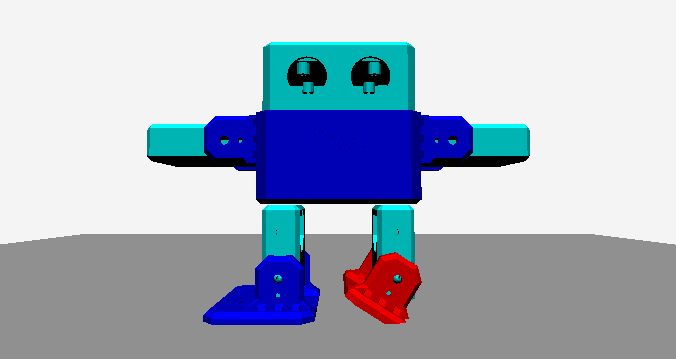
\includegraphics[width=0.4\textwidth]{images/otto-without-collision}}
\caption[Robot Otto - simulácia bez detekcie kolízií]{Robot Otto - simulácia bez detekcie kolízií}
\label{obr:otto-without-collision}
\end{figure}

\begin{figure}
\centerline{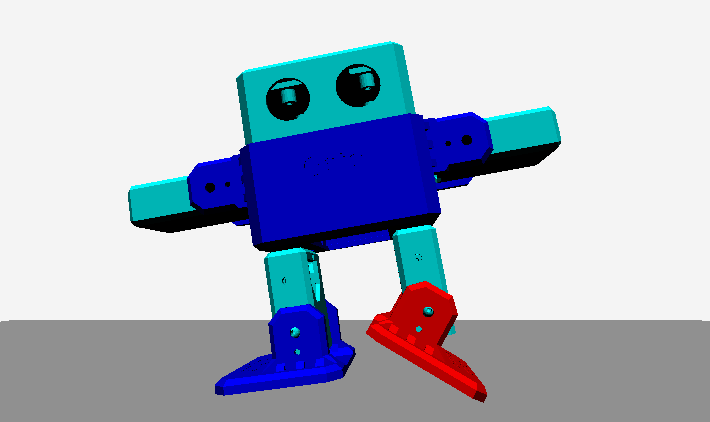
\includegraphics[width=0.4\textwidth]{images/otto-with-collision}}
\caption[Robot Otto - simulácia s detekciou kolízií]{Robot Otto - simulácia s detekciou kolízií}
\label{obr:otto-with-collision}
\end{figure}


%%%%%
% %%%    Riadiaci program robota
%%%%%
\section{Riadiaci program robota}
todo












